\documentclass[12pt, a4paper, oneside]{ctexart}
\usepackage{amsmath, amsthm, amssymb, bm, color, graphicx, geometry, mathrsfs,extarrows, braket, booktabs, array}
\usepackage[colorlinks,linkcolor=red,anchorcolor=blue,citecolor=blue,urlcolor=blue,menucolor=black]{hyperref}
\setmainfont{Times New Roman}  % 设置英文字体
\setsansfont{Calibri}
\setmonofont{Consolas}

\linespread{1.4}
%\geometry{left=2.54cm,right=2.54cm,top=3.18cm,bottom=3.18cm}
\geometry{left=1.84cm,right=1.84cm,top=2.18cm,bottom=2.18cm}
\newenvironment{problem}{\par\noindent\textbf{题目. }}{\bigskip\par}
\newenvironment{solution}{\par\noindent\textbf{解答. }}{\bigskip\par}
\newenvironment{note}{\par\noindent\textbf{注记. }}{\bigskip\par}

%%%% 图片相对路径 %%%%
\graphicspath{{figure/}} % 当前目录下的figure文件夹, {../figure/}则是父目录的figure文件夹

\everymath{\displaystyle} % 默认全部行间公式
\DeclareMathOperator*\uplim{\overline{lim}} % 定义上极限 \uplim_{}
\DeclareMathOperator*\lowlim{\underline{lim}} % 定义下极限 \lowlim_{}
\let\leq=\leqslant % 将全部leq变为leqslant
\let\geq=\geqslant % geq同理

% 一些宏定义
\def\bd{\boldsymbol}        % 加粗(向量) boldsymbol
\def\disp{\displaystyle}    % 使用行间公式 displaystyle(默认)
\def\tsty{\textstyle}       % 使用行内公式 textstyle
\def\sign{\text{sign}}      % sign function
\def\wtd{\widetilde}        % 宽波浪线 widetilde
\def\R{\mathbb{R}}          % Real number
\def\N{\mathbb{N}}          % Natural number
\def\Z{\mathbb{Z}}          % Integer number
\def\C{\mathbb{C}}          % Complex number
\def\d{\mathrm{d}}          % differential operator
\def\e{\mathrm{e}}          % Euler's number
\def\i{\mathrm{i}}          % imaginary number
\def\re{\mathrm{Re}}        % Real part
\def\im{\mathrm{Im}}        % Imaginary part
\def\res{\mathrm{Res}}      % Residue
\def\L{\mathcal{L}}         % Loss function
\def\wdh{\widehat}          % 宽帽子 widehat
\def\ol{\overline}          % 上横线 overline
\def\ul{\underline}         % 下横线 underline
\def\add{\vspace{1ex}}      % 增加行间距
\def\del{\vspace{-3.5ex}}   % 减少行间距
\def\bf{\textbf}

% 基本信息
\newcommand{\RQ}{\today} % 日期
\newcommand{\km}{实变函数} % 科目
\newcommand{\bj}{强基数学002} % 班级
\newcommand{\xm}{吴天阳} % 姓名
\newcommand{\xh}{2204210460} % 学号

\begin{document}

% 正文部分
\section*{基本概念}

数据的基本单元: \bf{数据元素}.

数据(元素)的最小单元: \bf{数据项}(不可分割).

数据结构: 分为\bf{逻辑结构}和\bf{存储(物理)结构}.

存储(物理)结构: \bf{顺序存储、链式存储、索引存储、散列存储}.

评价一个算法的两个标准: \bf{时间复杂度$T(n)$、空间复杂度$S(n)$}.

数据结构研究的三个方面: \bf{逻辑结构、存储结构、算法}.

\bf{线性结构}: 元素之间的逻辑关系用\ul{线性序列简单表示}.

\bf{非线性结构}: 不是线性结构(顾名思义).

\bf{头指针}: 指向链表中的第一个结点(头结点或首元结点)的指针.

\bf{首元结点}: 是第一个数据元素结点(第一个用于存储数据的结点).

\bf{头结点}: 首元结点之前的一个结点(不用于存储数据, 只作为链表的开头).

\begin{figure}[htbp]
    \centering
    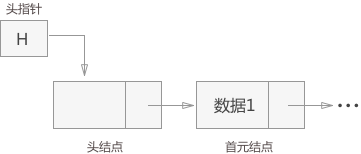
\includegraphics[scale=0.6]{头指针,头结点,首元结点区别.png}
    \caption{头指针, 头结点, 首元结点的区别}
\end{figure}

\bf{指针域}: 存储直接后继存储位置的域. (就是常用的next指针)

\bf{线性表包括}: 顺序表(数组), 链表(单链表, 双链表). (两者的优缺点可以对照记忆)

\bf{顺序优缺点}(a为优点, b为缺点): 

a.1. 具有\bf{随机存储特性}(注意区分它的\bf{存储单元是连续的一块}), 也可以说是可以\bf{直接访问}数据元素.

随机存储$=$直接访问$\neq$连续的存储单元.

a.2. \bf{存储密度大}, 无需为线性表中各元素间的逻辑关系而增加存储空间(省去了链表所需要存储的指针域, 以减少空间).

b.1. \bf{插入和删除操作时间复杂度高}, 需要移动大量元素.

b.2. \bf{初始空间不宜分配}(需要初始化数组必须给定一个大小).

\bf{链表优缺点}(a为优点, b为缺点): 

a.1. 采用\bf{动态分配}的方法, 内存利用率高. (用多少结点就创建多少个, 不多不少)

a.2. \bf{插入和删除操作时间复杂度低}, 只需修改指针域, 无需移动元素. (改下指针的指向即可)

b.1. \bf{存储密度小}, 记录元素之间的逻辑关系需要额外的存储空间. (需要记录指针域)

b.2. \bf{不具有随机存储特性}.

线性表和链表的使用场景: 如需要快速地读取且很少使用插入删除操作, 则使用顺序表; 如遇到需要频繁使用插入删除操作, 则用链表.



% 下面给一些功能的写法
\iffalse
% 图片模板
\centerline{
    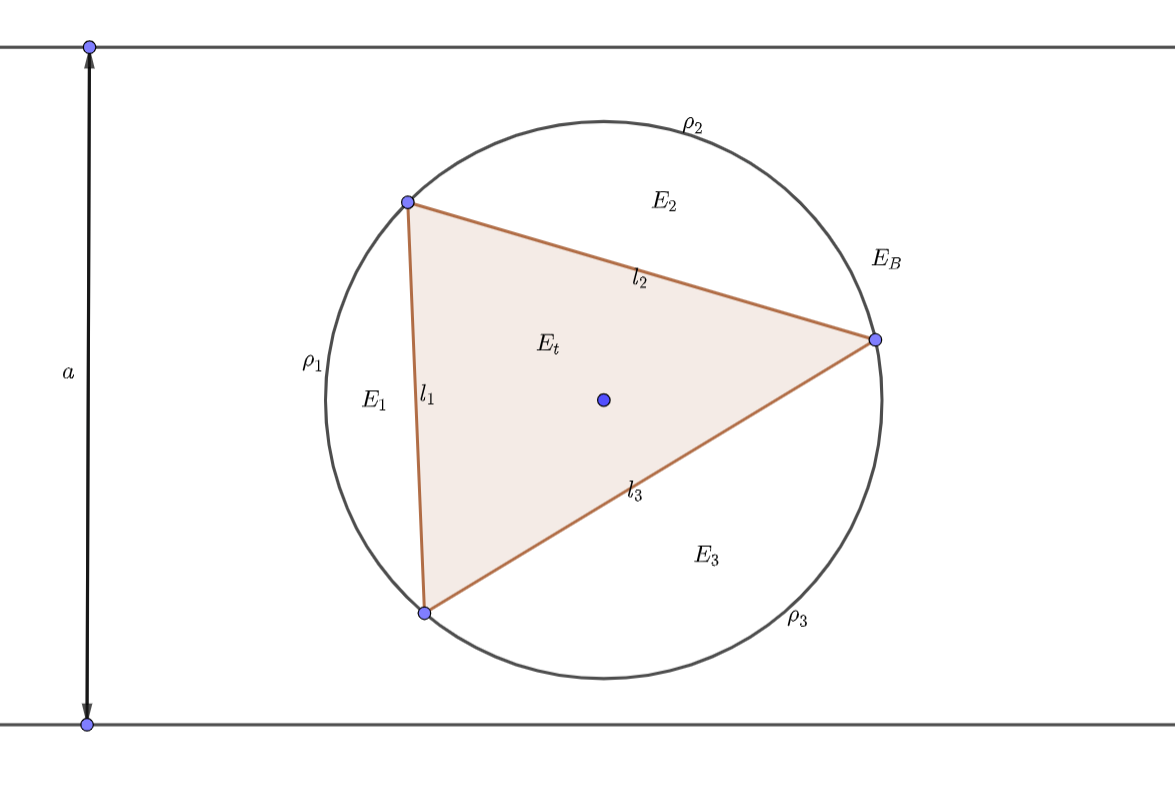
\includegraphics[width=0.8\textwidth]{figure.png}
}
% 表格模板
\renewcommand\arraystretch{0.8} % 设置表格高度为原来的0.8倍
\begin{table}[!htbp] % table标准
    \centering % 表格居中
    \begin{tabular}{p{1cm}<{\centering}p{1cm}<{\centering}p{3cm}<{\centering}p{5cm}<{\centering}} % 设置表格宽度
    %\begin{tabular}{cccc}
        \toprule
        $x_i$ & $f[x_1]$ & $f[x_i,x_{i+1}]$ & $f[x_i,x_{i+1},x_{i+2}]$ \\
        \midrule
        $x_0$ & $f(x_0)$ &                  &                          \\
        $x_0$ & $f(x_0)$ & $f'(x_0)$        &                          \\
        $x_0$ & $f(x_1)$ & $\frac{f(x_1)-f(x_0)}{x_1-x_0}$ & $\frac{f(x_1)-f(x_0)}{(x_1-x_0)^2}-\frac{f'(x_0)}{x_1-x_0}$\\
        \bottomrule
    \end{tabular}
\end{table}

\def\Log{\text{Log}} % 一个简单的宏定义
$\Log$ % 调用方法
\fi

\end{document}